\documentclass[11pt]{article}
\usepackage[latin1]{inputenc}
\usepackage{amsmath}
\usepackage{amsfonts}
\usepackage{amssymb}
\usepackage{graphicx}
\usepackage{setspace}
\usepackage[left=1.00in, right=1.00in, top=1.00in, bottom=1.00in]{geometry}
\usepackage[english]{babel}
\newcommand{\forceindent}{\leavevmode{\parindent=1.5em\indent}} % em = roughly width of uppercase ``M", or just over a third of a cm

\usepackage{fancyhdr}

\pagestyle{fancy}
\fancyhf{}
\rhead{University of Houston $|$ Political Science}
\lhead{Learning \LaTeX: Week 2} %% BE SURE TO CHANGE THIS EACH WEEK
\rfoot{Page \thepage}

\usepackage[round]{natbib}
\bibliographystyle{apsr}

\begin{document}
	
	\title{Learning \LaTeX \\
		\vspace{1cm}
	\large Week 2: Tables \& Graphics \\ %% BE SURE TO CHANGE EACH WEEK
		\vspace{1cm}}
	\author{Philip D. Waggoner\footnote{{\texttt{philip.waggoner@gmail.com}}. This document was prepared by Philip Waggoner for the \textit{Weekly Workshops on Learning \LaTeX}, hosted by the Deparment of Political Science, University of Houston.}}
	\date{ } % getting rid of the automatic date
	\maketitle

\newpage

\tableofcontents

\newpage

\section{Introductory Remarks}
	
\forceindent Drawing tables in \LaTeX\, like most other things, can be simple or quite difficult. The idea behind drawing tables is in line with doing anything else in \LaTeX\, where we need to start with environments, and then proceed to complicate as much as we like. \\

It can be frustrating to draw tables, becuase each cell must be in alignment, though there are no boundaries keeping each cell in place, like there is in Excel, for example. Thus, drawing tables requires meticulous care and attention. But the result is well-worth the trouble. \\

There are many different table environments in \LaTeX\ (e.g., table, tabular, tabu, tabularx, and so on). For today's purposes, and for most research, table and tabular should be sufficient. The difference between these two environments in that \textit{tabular} is the default table maker in \LaTeX, and \textit{table} allows for a ``floating" environment, where we can move tables around more efficiently and easily. We will be using each of these environments in today's workshop. \\

Our goals for today:

\begin{itemize}
	\item Draw and manipulate tables, positions, \& content
	\item Reference tables within text
	\item Insert notes within tables
	\item Insert graphics, plots, \& figures
\end{itemize}

\newpage 

\section{Tables}

\forceindent Let's get started with a simple table. To do so, we need to know a couple of useful commands and syntax. First, columns are generated by a position indicator such as ``c" (for ``center", or ``l", ``r" and so on), cell delineators are generated by ``$|$", horizontal lines are inserted into the table with the command ``hline", and we tell \LaTeX\ where to put our values with the use of the ampersand, ``\&". \\

Thus, for a simple table, let's start with the following code,

\begin{figure}[!h]
	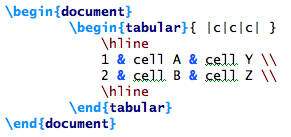
\includegraphics[scale=.5]{CODE1} \\ %[width=12cm, height=11cm] % to use instead of scale if need be
	%\centering
\end{figure}

And this code gives us,

\begin{figure}[!h]
	
\includegraphics[scale=.6]{OUT1} \\ %[width=12cm, height=11cm] % to use instead of scale if need be
	\centering
\end{figure}

So from the output, we can see that we told \LaTeX\ to generate a table with three columns, with dividing lines between each column. And there should be two rows, given the two rows of information we provided. Let's change some of these parameters to see how the simple table changes. Specifically, let's add another line on top of the table, addional lines on the ends, but remove the column dividers within the table, and let's also add another row of information. \\

Try this new code, 

\begin{figure}[!h]
	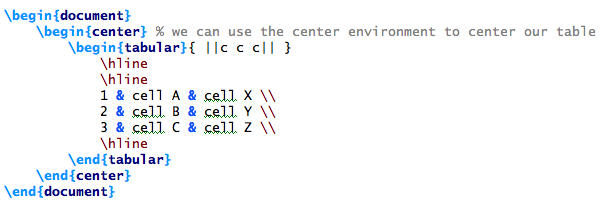
\includegraphics[scale=.5]{CODE2} \\ %[width=12cm, height=11cm] % to use instead of scale if need be
	%\centering
\end{figure}

Now our table looks like,

\begin{figure}[!h]
	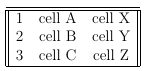
\includegraphics[scale=.6]{OUT2} \\ %[width=12cm, height=11cm] % to use instead of scale if need be
	\centering
\end{figure}

\subsection{Combining Columns}

\forceindent Now that we have the basic intuition behind creating a table, let's complicate things just a little to give us more flexibility for customizing tables. We will start by combining columns in only part of the table. To do so, we need a new command, ``multicolumn". This means, then, that we will also need to add a new line to our original table. Let's start with the following code,

\begin{figure}[!h]
	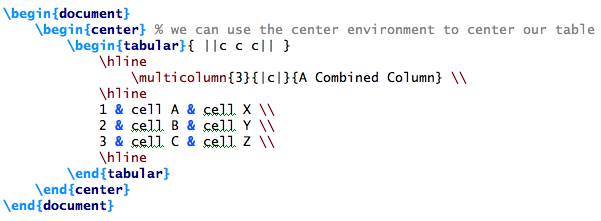
\includegraphics[scale=.5]{CODE3} \\ %[width=12cm, height=11cm] % to use instead of scale if need be
	%\centering
\end{figure}

Then, we get the updated table,

\begin{figure}[!h]
	
\includegraphics[scale=.6]{OUT3} \\ %[width=12cm, height=11cm] % to use instead of scale if need be
	\centering
\end{figure}

We can see our new table has a new row added to the top of the table, which is comprised of three columns. This is useful for delineating between different models presented in a single table, for example. We can also combine several columns within the table, rather than the full length of the table. So for our simple table, 

\begin{figure}[!h]
	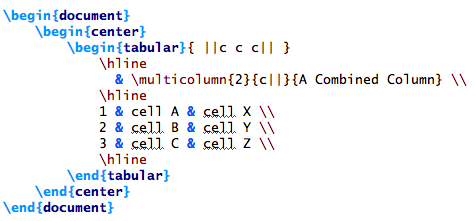
\includegraphics[scale=.5]{CODE4} \\ %[width=12cm, height=11cm] % to use instead of scale if need be
	%\centering
\end{figure}

\newpage

And our output looks like,

\begin{figure}[!h]
	
\includegraphics[scale=.6]{OUT4} \\ %[width=12cm, height=11cm] % to use instead of scale if need be
	\centering
\end{figure}

Notice the combined two columns over the right two columns in the table. This is possible through the addition of the ``\{2\}\{c$|$$|$\}", which tells multicolumn to combine only 2 columns, even though there are three, and then to place the double lines to the right of it, to be consistent with our table format. Also notice the blank space in front of the \& in the multicolumn line. This tells the tabular environment to not place anything in  that space, but to still include it as a column in the table.


\subsection{Position Tables Using the ``Table" Environment}

\forceindent To this point, we have only been using the tabular environment to draw a table in \LaTeX. But let's say we want more flexibility over precisely where our table is placed in the body of the text. The default position using only the tabular environment, is exactly where you insert the code. Thus, the table environment lets us specify the table's location. \\

To get started, we simply nest the tabular table within the table environment, and then specify the location using brackets after ``table", and then one of the following positional identifiers: h (``here"), t (``top"), b (``bottom"), p (specific ``page"), ! (``override internal position from \LaTeX), H (``exactly here", which also equals, ``h!"). To update our simple table code, type,

\begin{figure}[!h]
	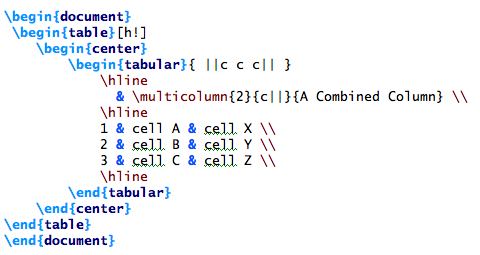
\includegraphics[scale=.5]{CODE5} \\ %[width=12cm, height=11cm] % to use instead of scale if need be
	%\centering
\end{figure}

And here's the output, 

\begin{figure}[!h]
	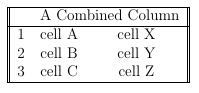
\includegraphics[scale=.6]{OUT5} \\ %[width=12cm, height=11cm] % to use instead of scale if need be
	\centering
\end{figure}

But, to see the precise impact of these positional identifiers, let's see all positions at once. Try several of them back to back,

\begin{figure}[!h]
	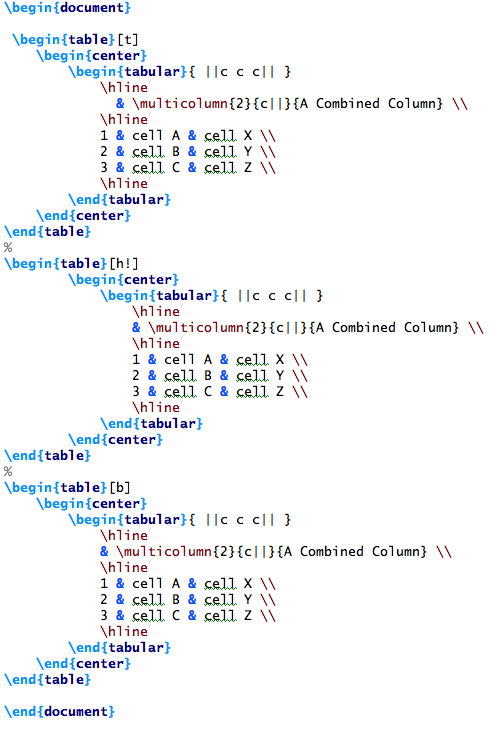
\includegraphics[scale=.5]{CODE6} \\ %[width=12cm, height=11cm] % to use instead of scale if need be
	%\centering
\end{figure}

\newpage

And here's the output,

\begin{figure}[!h]
	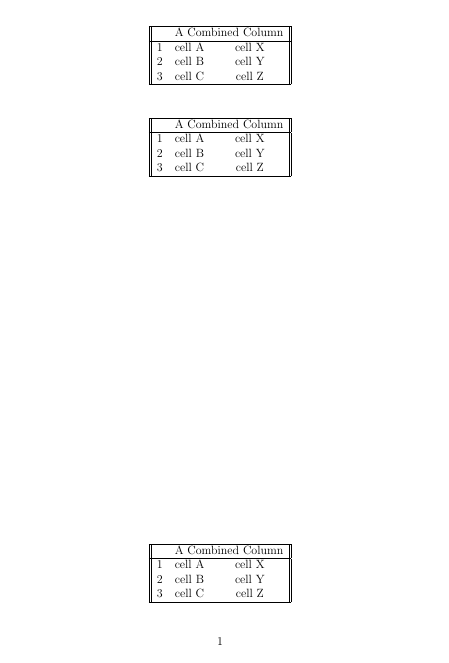
\includegraphics[scale=.6]{OUT6} \\ %[width=12cm, height=11cm] % to use instead of scale if need be
	\centering
\end{figure}

\newpage

\subsection{Captions, Labels, \& In-Text Referencing}

\forceindent One of the best features of \LaTeX\ is the ability to keep track of all tables, figures, and equations, regardless of how the text may change. For example, let's say you have a document with four tables in it. But you update the paper and decide you need to add a table of descriptive statistics. So instead of having to go back and manually change all table numbers, and also change any place in the text you reference the old table numbers, \LaTeX\ allows you to imply reference the table with an in-text command based on the caption you gave the table. Thus, adding this fifth table is no problem at all. Nothing in your text changes, and \LaTeX\ does the work of updating all references to table as well as table numbers throughout your text. \\

To get a better sense of this, we need to use the ``caption" and ``label" commands. The caption command gives the table a name, which is attached to the table wherever it goes in the text. The label command provides the reference we can cite within the text to keep us on track with our table numbering. To actually cite within the text, we type ``ref" after the backslash to call the reference command. \\

So let's update some code for two tables in order to see precisely how these commands work. Type,

\begin{figure}[!h]
	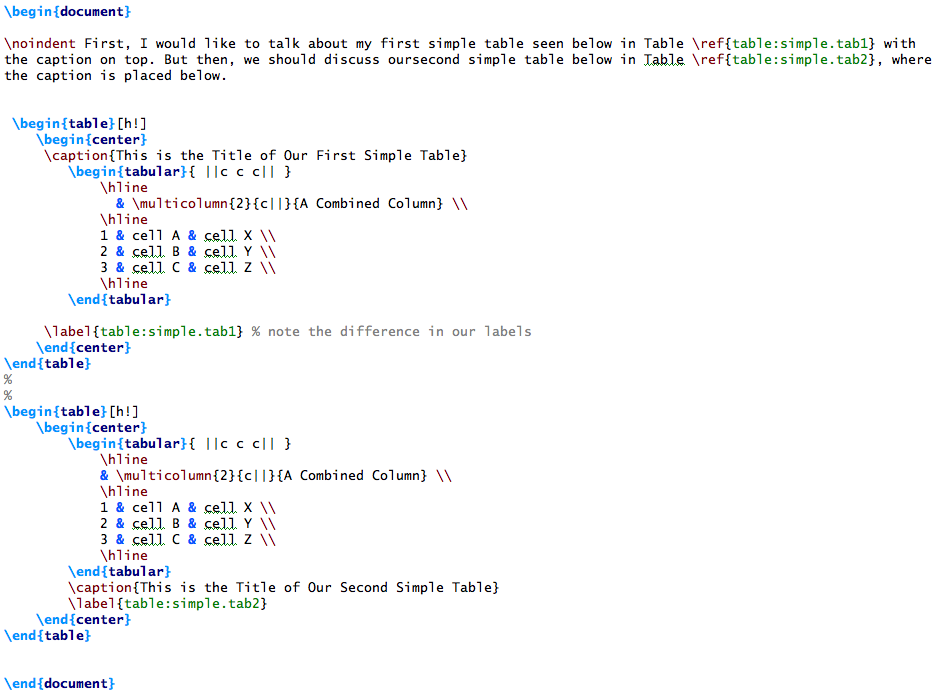
\includegraphics[scale=.5]{CODE7} \\ %[width=12cm, height=11cm] % to use instead of scale if need be
	%\centering
\end{figure}

\newpage

Then, we can see the ouput as,

\begin{figure}[!h]
	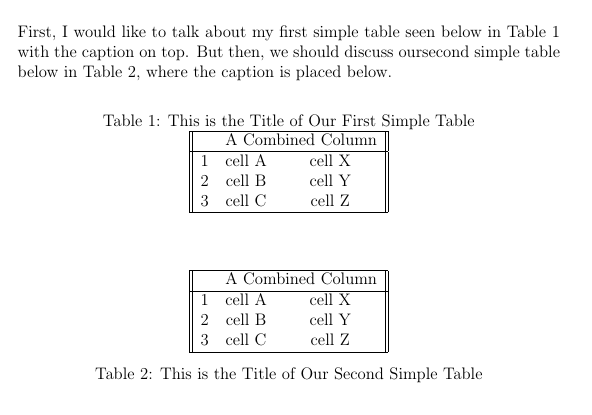
\includegraphics[scale=.6]{OUT7} \\ %[width=12cm, height=11cm] % to use instead of scale if need be
	\centering
\end{figure}

\subsection{Table Notes}

\forceindent Finally, you almost always see some kind of note at the bottom of a table (e.g., denoting levels of statistical significance, references to standard errors, and so on). There are many ways to do this (e.g., threeparttable - you should look this up and use it on your own), but the simplest way for our purposes, is to add subsequent lines to the bottom of our table and manually format to resemble a proper table footnote using our multicolumn command from earlier, where the syntax following the multicolumn command is, ``\{columns\}\{position\}\{text\}." \\

To do this, let's update our code to make our simple table look a little nicer with our new footnote,

\begin{figure}[!h]
	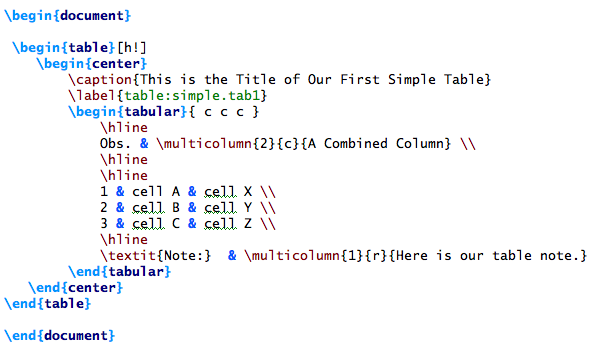
\includegraphics[scale=.5]{CODE8} \\ %[width=12cm, height=11cm] % to use instead of scale if need be
	%\centering
\end{figure}

\newpage

Now, we can see our updated table is starting to look a bit more like something we would see in a journal (though we still have a ways to go),\footnote{In \texttt{R}, we can generate base tables of results very easily in many ways. The two main ways to get you started are using either ``stargazer" or ``xtable" packages. In stargazer, you can simultaneously print and save results, while also generating \LaTeX\ code to simply copy and paste into \LaTeX. In xtable, you can print the \LaTeX\ code as well.}

\begin{figure}[!h]
	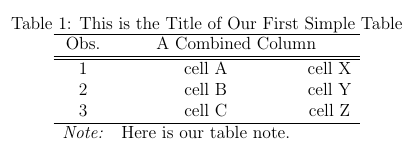
\includegraphics[scale=.6]{OUT8} \\ %[width=12cm, height=11cm] % to use instead of scale if need be
	\centering
\end{figure}


\newpage


\section{Graphics, Plots, \& Pictures}

\forceindent To conclude, we will take a look at inserting and manipulating figures/plots/graphics/images (hereafter, \textit{images}) into a \LaTeX\ document. First, \textit{we must save all images in the same location as our main \TeX\ document}. So for example, if we have a paper saved in the folder called, ``Class 1 Final Paper," all images we want to include in that paper for Class 1 must also be saved in the the ``Class 1 Final Paper" folder. Once we have saved all images in the same location, we need to now need to load a package called ``graphicx." This let's us place images in a file, as well as allows us to tell \LaTeX\ where to track down our images. Once the package is included in our preamble (at the top of our \TeX\ document), below it we need to set the ``graphicspath." This is simply the file path to the location of your main document, set within braces, which specifies the location of both your main document and your images. The synax would look like,

\begin{figure}[!h]
	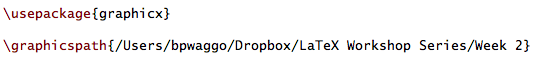
\includegraphics[scale=.5]{CODE9} \\ %[width=12cm, height=11cm] % to use instead of scale if need be
	%\centering
\end{figure}

Once we have our preamble set, and our graphics path specified, we can now insert images easily into any location in our paper using the ``figure" environment.\footnote{You can simply use the command ``includegraphics." But this limits our flexibility for manipulating the image as we see fit. Thus, let's focus on using the figure environment instead.} The figure environment, like the ``table" environment, allows us to specify precisely where we want to place our images using the same positional identifiers (e.g., \textit{h}, \textit{t}, \textit{b}, etc.). \\

Let's first go to the internet and find an image of anything you want to include in your document. Once you have this, place it in the same location as your main document, whereever that is. Then, to call and place this image, we simply type,

\begin{figure}[!h]
	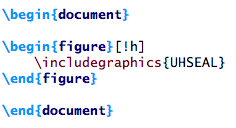
\includegraphics[scale=.5]{CODE10} \\ %[width=12cm, height=11cm] % to use instead of scale if need be
	%\centering
\end{figure}

\newpage

Then, our output is the image,

\begin{figure}[!h]
	
\includegraphics[scale=.4]{OUT10} \\ %[width=12cm, height=11cm] % to use instead of scale if need be
	\centering
\end{figure}

\subsection{A Few Notes on Scaling \& Sizing}

\forceindent Now there are a few things to consider here. First, I always make the names of my files as simple and clear as possible to limit the threat of confusing \LaTeX, such as removing file types from the title (.png, etc.). Also, for our purposes, let's stick with only .png files. Its cleaner and easier for the figure environment, though we can include other image types. As we are using the figure environment, we can manipulate the alignment of the opbject as with a table, using commands such as ``center" (see above on centering our tables). Also, and importantly, notice how our image is a little fuzzy. This can easily be corrected by either changing the dimensions of height and width of the image manually using brackets just after the ``includegraphics" command (e.g., ``width=12cm, height=11cm"), or for a more careful and simpler fix, we can simply alter the scale of the image. To get a sense of this, let's update our code with a few options of rescaling,

\begin{figure}[!h]
	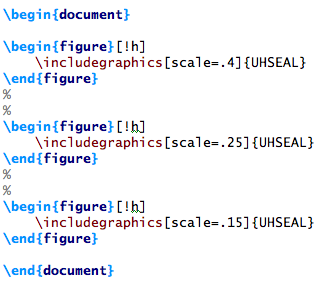
\includegraphics[scale=.5]{CODE11} \\ %[width=12cm, height=11cm] % to use instead of scale if need be
	%\centering
\end{figure}

\newpage

Now, let's see each of the three iterations of the rescaled University of Houston seal,

\begin{figure}[!h]
	
\includegraphics[scale=.4]{OUT11} \\ %[width=12cm, height=11cm] % to use instead of scale if need be
	\centering
\end{figure}

\end{document}
